
%% bare_conf.tex
%% V1.4b
%% 2015/08/26
%% by Michael Shell
%% See:
%% http://www.michaelshell.org/
%% for current contact information.
%%
%% This is a skeleton file demonstrating the use of IEEEtran.cls
%% (requires IEEEtran.cls version 1.8b or later) with an IEEE
%% conference paper.
%%
%% Support sites:
%% http://www.michaelshell.org/tex/ieeetran/
%% http://www.ctan.org/pkg/ieeetran
%% and
%% http://www.ieee.org/

%%*************************************************************************
%% Legal Notice:
%% This code is offered as-is without any warranty either expressed or
%% implied; without even the implied warranty of MERCHANTABILITY or
%% FITNESS FOR A PARTICULAR PURPOSE! 
%% User assumes all risk.
%% In no event shall the IEEE or any contributor to this code be liable for
%% any damages or losses, including, but not limited to, incidental,
%% consequential, or any other damages, resulting from the use or misuse
%% of any information contained here.
%%
%% All comments are the opinions of their respective authors and are not
%% necessarily endorsed by the IEEE.
%%
%% This work is distributed under the LaTeX Project Public License (LPPL)
%% ( http://www.latex-project.org/ ) version 1.3, and may be freely used,
%% distributed and modified. A copy of the LPPL, version 1.3, is included
%% in the base LaTeX documentation of all distributions of LaTeX released
%% 2003/12/01 or later.
%% Retain all contribution notices and credits.
%% ** Modified files should be clearly indicated as such, including  **
%% ** renaming them and changing author support contact information. **
%%*************************************************************************


% *** Authors should verify (and, if needed, correct) their LaTeX system  ***
% *** with the testflow diagnostic prior to trusting their LaTeX platform ***
% *** with production work. The IEEE's font choices and paper sizes can   ***
% *** trigger bugs that do not appear when using other class files.       ***                          ***
% The testflow support page is at:
% http://www.michaelshell.org/tex/testflow/



\documentclass[conference]{IEEEtran}
% Some Computer Society conferences also require the compsoc mode option,
% but others use the standard conference format.
%
% If IEEEtran.cls has not been installed into the LaTeX system files,
% manually specify the path to it like:
% \documentclass[conference]{../sty/IEEEtran}





% Some very useful LaTeX packages include:
% (uncomment the ones you want to load)


% *** MISC UTILITY PACKAGES ***
%
%\usepackage{ifpdf}
% Heiko Oberdiek's ifpdf.sty is very useful if you need conditional
% compilation based on whether the output is pdf or dvi.
% usage:
% \ifpdf
%   % pdf code
% \else
%   % dvi code
% \fi
% The latest version of ifpdf.sty can be obtained from:
% http://www.ctan.org/pkg/ifpdf
% Also, note that IEEEtran.cls V1.7 and later provides a builtin
% \ifCLASSINFOpdf conditional that works the same way.
% When switching from latex to pdflatex and vice-versa, the compiler may
% have to be run twice to clear warning/error messages.






% *** CITATION PACKAGES ***
%
%\usepackage{cite}
% cite.sty was written by Donald Arseneau
% V1.6 and later of IEEEtran pre-defines the format of the cite.sty package
% \cite{} output to follow that of the IEEE. Loading the cite package will
% result in citation numbers being automatically sorted and properly
% "compressed/ranged". e.g., [1], [9], [2], [7], [5], [6] without using
% cite.sty will become [1], [2], [5]--[7], [9] using cite.sty. cite.sty's
% \cite will automatically add leading space, if needed. Use cite.sty's
% noadjust option (cite.sty V3.8 and later) if you want to turn this off
% such as if a citation ever needs to be enclosed in parenthesis.
% cite.sty is already installed on most LaTeX systems. Be sure and use
% version 5.0 (2009-03-20) and later if using hyperref.sty.
% The latest version can be obtained at:
% http://www.ctan.org/pkg/cite
% The documentation is contained in the cite.sty file itself.
\usepackage{graphicx}






% *** GRAPHICS RELATED PACKAGES ***
%
\ifCLASSINFOpdf
  % \usepackage[pdftex]{graphicx}
  % declare the path(s) where your graphic files are
  % \graphicspath{{../pdf/}{../jpeg/}}
  % and their extensions so you won't have to specify these with
  % every instance of \includegraphics
  % \DeclareGraphicsExtensions{.pdf,.jpeg,.png}
\else
  % or other class option (dvipsone, dvipdf, if not using dvips). graphicx
  % will default to the driver specified in the system graphics.cfg if no
  % driver is specified.
  % \usepackage[dvips]{graphicx}
  % declare the path(s) where your graphic files are
  % \graphicspath{{../eps/}}
  % and their extensions so you won't have to specify these with
  % every instance of \includegraphics
  % \DeclareGraphicsExtensions{.eps}
\fi
% graphicx was written by David Carlisle and Sebastian Rahtz. It is
% required if you want graphics, photos, etc. graphicx.sty is already
% installed on most LaTeX systems. The latest version and documentation
% can be obtained at: 
% http://www.ctan.org/pkg/graphicx
% Another good source of documentation is "Using Imported Graphics in
% LaTeX2e" by Keith Reckdahl which can be found at:
% http://www.ctan.org/pkg/epslatex
%
% latex, and pdflatex in dvi mode, support graphics in encapsulated
% postscript (.eps) format. pdflatex in pdf mode supports graphics
% in .pdf, .jpeg, .png and .mps (metapost) formats. Users should ensure
% that all non-photo figures use a vector format (.eps, .pdf, .mps) and
% not a bitmapped formats (.jpeg, .png). The IEEE frowns on bitmapped formats
% which can result in "jaggedy"/blurry rendering of lines and letters as
% well as large increases in file sizes.
%
% You can find documentation about the pdfTeX application at:
% http://www.tug.org/applications/pdftex





% *** MATH PACKAGES ***
%
%\usepackage{amsmath}
% A popular package from the American Mathematical Society that provides
% many useful and powerful commands for dealing with mathematics.
%
% Note that the amsmath package sets \interdisplaylinepenalty to 10000
% thus preventing page breaks from occurring within multiline equations. Use:
%\interdisplaylinepenalty=2500
% after loading amsmath to restore such page breaks as IEEEtran.cls normally
% does. amsmath.sty is already installed on most LaTeX systems. The latest
% version and documentation can be obtained at:
% http://www.ctan.org/pkg/amsmath





% *** SPECIALIZED LIST PACKAGES ***
%
%\usepackage{algorithmic}
% algorithmic.sty was written by Peter Williams and Rogerio Brito.
% This package provides an algorithmic environment fo describing algorithms.
% You can use the algorithmic environment in-text or within a figure
% environment to provide for a floating algorithm. Do NOT use the algorithm
% floating environment provided by algorithm.sty (by the same authors) or
% algorithm2e.sty (by Christophe Fiorio) as the IEEE does not use dedicated
% algorithm float types and packages that provide these will not provide
% correct IEEE style captions. The latest version and documentation of
% algorithmic.sty can be obtained at:
% http://www.ctan.org/pkg/algorithms
% Also of interest may be the (relatively newer and more customizable)
% algorithmicx.sty package by Szasz Janos:
% http://www.ctan.org/pkg/algorithmicx




% *** ALIGNMENT PACKAGES ***
%
%\usepackage{array}
% Frank Mittelbach's and David Carlisle's array.sty patches and improves
% the standard LaTeX2e array and tabular environments to provide better
% appearance and additional user controls. As the default LaTeX2e table
% generation code is lacking to the point of almost being broken with
% respect to the quality of the end results, all users are strongly
% advised to use an enhanced (at the very least that provided by array.sty)
% set of table tools. array.sty is already installed on most systems. The
% latest version and documentation can be obtained at:
% http://www.ctan.org/pkg/array


% IEEEtran contains the IEEEeqnarray family of commands that can be used to
% generate multiline equations as well as matrices, tables, etc., of high
% quality.




% *** SUBFIGURE PACKAGES ***
%\ifCLASSOPTIONcompsoc
%  \usepackage[caption=false,font=normalsize,labelfont=sf,textfont=sf]{subfig}
%\else
%  \usepackage[caption=false,font=footnotesize]{subfig}
%\fi
% subfig.sty, written by Steven Douglas Cochran, is the modern replacement
% for subfigure.sty, the latter of which is no longer maintained and is
% incompatible with some LaTeX packages including fixltx2e. However,
% subfig.sty requires and automatically loads Axel Sommerfeldt's caption.sty
% which will override IEEEtran.cls' handling of captions and this will result
% in non-IEEE style figure/table captions. To prevent this problem, be sure
% and invoke subfig.sty's "caption=false" package option (available since
% subfig.sty version 1.3, 2005/06/28) as this is will preserve IEEEtran.cls
% handling of captions.
% Note that the Computer Society format requires a larger sans serif font
% than the serif footnote size font used in traditional IEEE formatting
% and thus the need to invoke different subfig.sty package options depending
% on whether compsoc mode has been enabled.
%
% The latest version and documentation of subfig.sty can be obtained at:
% http://www.ctan.org/pkg/subfig




% *** FLOAT PACKAGES ***
%
%\usepackage{fixltx2e}
% fixltx2e, the successor to the earlier fix2col.sty, was written by
% Frank Mittelbach and David Carlisle. This package corrects a few problems
% in the LaTeX2e kernel, the most notable of which is that in current
% LaTeX2e releases, the ordering of single and double column floats is not
% guaranteed to be preserved. Thus, an unpatched LaTeX2e can allow a
% single column figure to be placed prior to an earlier double column
% figure.
% Be aware that LaTeX2e kernels dated 2015 and later have fixltx2e.sty's
% corrections already built into the system in which case a warning will
% be issued if an attempt is made to load fixltx2e.sty as it is no longer
% needed.
% The latest version and documentation can be found at:
% http://www.ctan.org/pkg/fixltx2e


%\usepackage{stfloats}
% stfloats.sty was written by Sigitas Tolusis. This package gives LaTeX2e
% the ability to do double column floats at the bottom of the page as well
% as the top. (e.g., "\begin{figure*}[!b]" is not normally possible in
% LaTeX2e). It also provides a command:
%\fnbelowfloat
% to enable the placement of footnotes below bottom floats (the standard
% LaTeX2e kernel puts them above bottom floats). This is an invasive package
% which rewrites many portions of the LaTeX2e float routines. It may not work
% with other packages that modify the LaTeX2e float routines. The latest
% version and documentation can be obtained at:
% http://www.ctan.org/pkg/stfloats
% Do not use the stfloats baselinefloat ability as the IEEE does not allow
% \baselineskip to stretch. Authors submitting work to the IEEE should note
% that the IEEE rarely uses double column equations and that authors should try
% to avoid such use. Do not be tempted to use the cuted.sty or midfloat.sty
% packages (also by Sigitas Tolusis) as the IEEE does not format its papers in
% such ways.
% Do not attempt to use stfloats with fixltx2e as they are incompatible.
% Instead, use Morten Hogholm'a dblfloatfix which combines the features
% of both fixltx2e and stfloats:
%
% \usepackage{dblfloatfix}
% The latest version can be found at:
% http://www.ctan.org/pkg/dblfloatfix




% *** PDF, URL AND HYPERLINK PACKAGES ***
%
%\usepackage{url}
% url.sty was written by Donald Arseneau. It provides better support for
% handling and breaking URLs. url.sty is already installed on most LaTeX
% systems. The latest version and documentation can be obtained at:
% http://www.ctan.org/pkg/url
% Basically, \url{my_url_here}.




% *** Do not adjust lengths that control margins, column widths, etc. ***
% *** Do not use packages that alter fonts (such as pslatex).         ***
% There should be no need to do such things with IEEEtran.cls V1.6 and later.
% (Unless specifically asked to do so by the journal or conference you plan
% to submit to, of course. )


% correct bad hyphenation here
\hyphenation{op-tical net-works semi-conduc-tor}


\begin{document}
%
% paper title
% Titles are generally capitalized except for words such as a, an, and, as,
% at, but, by, for, in, nor, of, on, or, the, to and up, which are usually
% not capitalized unless they are the first or last word of the title.
% Linebreaks \\ can be used within to get better formatting as desired.
% Do not put math or special symbols in the title.
\title{Normalised LMS Algorithm - Interference Cancelling, Project 1}


% author names and affiliations
% use a multiple column layout for up to three different
% affiliations
\author{\IEEEauthorblockN{Madhusudan Govindraju	}
\IEEEauthorblockA{
University of Florida\\
Email: madhusudangr@ufl.edu}
}

% conference papers do not typically use \thanks and this command
% is locked out in conference mode. If really needed, such as for
% the acknowledgment of grants, issue a \IEEEoverridecommandlockouts
% after \documentclass

% for over three affiliations, or if they all won't fit within the width
% of the page, use this alternative format:
% 
%\author{\IEEEauthorblockN{Michael Shell\IEEEauthorrefmark{1},
%Homer Simpson\IEEEauthorrefmark{2},
%James Kirk\IEEEauthorrefmark{3}, 
%Montgomery Scott\IEEEauthorrefmark{3} and
%Eldon Tyrell\IEEEauthorrefmark{4}}
%\IEEEauthorblockA{\IEEEauthorrefmark{1}School of Electrical and Computer Engineering\\
%Georgia Institute of Technology,
%Atlanta, Georgia 30332--0250\\ Email: see http://www.michaelshell.org/contact.html}
%\IEEEauthorblockA{\IEEEauthorrefmark{2}Twentieth Century Fox, Springfield, USA\\
%Email: homer@thesimpsons.com}
%\IEEEauthorblockA{\IEEEauthorrefmark{3}Starfleet Academy, San Francisco, California 96678-2391\\
%Telephone: (800) 555--1212, Fax: (888) 555--1212}
%\IEEEauthorblockA{\IEEEauthorrefmark{4}Tyrell Inc., 123 Replicant Street, Los Angeles, California 90210--4321}}




% use for special paper notices
%\IEEEspecialpapernotice{(Invited Paper)}




% make the title area
\maketitle

% As a general rule, do not put math, special symbols or citations
% in the abstract
\begin{abstract}
This papers gives a detailed report on how the problem statement for the project has been handled, with the assumptions and the learnings. The problem statement is an application of Normalized LMS algorithm to remove the noise from an audio signal. The problem also states that the input signal is 21KHz. We are to design and evaluate the performance of an adaptive FIR filter using the NLMS algorithm. This is also considered as an inference cancelling problem.

\end{abstract}

% no keywords




% For peer review papers, you can put extra information on the cover
% page as needed:
% \ifCLASSOPTIONpeerreview
% \begin{center} \bfseries EDICS Category: 3-BBND \end{center}
% \fi
%
% For peerreview papers, this IEEEtran command inserts a page break and
% creates the second title. It will be ignored for other modes.
\IEEEpeerreviewmaketitle



\section{Introduction}
With wiener solutions there are methods which explains, when the reference input is free of signal noise in the primary input can be cancelled without any or very less signal distortion\cite{AdaptiveNoiseCancelling1975}. There are various applications for adaptive noise cancelling in the industry, some of them include cancelling interference in the ECG, speech signal, borad-band interference in an antenna array \cite{AdaptiveNoiseCancelling1975}. The paper \cite{AdaptiveNoiseCancelling1975} also talks about the design of the filter to be used. We can use a fixed filter for this problem of noise cancelling if we have prior knowledge of both the signal and the noise. But adaptive filters will adjust their own parameters automatically, without prior knowledge of the signal or noise. One famous commercial application of adaptive filtering is the MODEM for digital communication, which are widely used in connecting computers through the internet with less interference. 

\section{Literature Review}

The earliest works in noise cancelling for Adaptive filters were "P.Howells, Intermediate frequency side-lobe canceller"\cite{Howells_SideLobeCanceller},"B.Widrow \& M.Hoff Adaptive Switching circuits"  \cite{WidrowHoffdaptiveSwitching}, "N.Nilsson, Learning Machines" \cite{McgrawhillNilssonLearningMachines}. 
Widrow and Hoff talk about an adaptive algorithm and pattern recognition scheme called the "Adaline" - short for "Adaptive  Linear Threshold Logic Element" in \cite{WidrowHoffdaptiveSwitching}. 


\section{Adaptive Filtering}

The basic model for adaptive filtering is shown in figure \ref{AdaptiveFilterBlockDiagram}. The $X(n)$ is the input signal and we need to predict the $Y(n)$. The desired output signal is denoted as $d(n)$ in the adder. The error between the desired and the obtained output signal will give rise to an error signal, based on this error signal the parameters of the adaptive algorithm are changed to give the $w(n+1)$ from the formula 

$$ w(n+1) = w(n) + StepSize * Error * X(n)  $$

where $w(n+1)$ is the new parameter and the $w(n)$ is the old parameter. This special adaptive filter is referred to as the LMS algorithm. To control the deviation caused due to the change in power of signal in real time we can normalize the signal with the power of the input signal to get the NLMS - Normalized LMS algorithm. \\

The equations to explain the Normalized LMS algorithm is as follows.


$$ Y = W^{T} \times  X$$
$$ Error = Desired - Y $$
$$ w(n+1) = w(n) + [StepSize/X(n) *X(n)'] * Error * X(n)  $$ \\

"NLMS is an iterative gradient descent algorithm that uses an estimate of the gradient on the mean square error surface to seek the minimum optimum weight vector at the minimum mean square error point. "\cite{GloverAdaptiveNoiseCancelling}

So this system actually corrects itself to learn from the error signal produced. So after a few iterations when the error signal goes to zero the desired output is approximately equal to the obtained output leading to a system which predicts exactly what we need. 
 
When we look a the convergence performance of the Normalized LMS algorithm, we can see that the normalized algorithm will adapt to the system in far fewer iterations.
 
 
 \begin{figure}
\centering
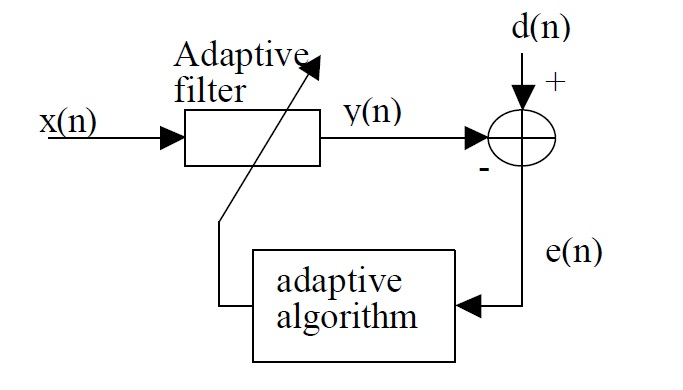
\includegraphics[width=2.5in]{image5.jpg}
\caption{Basic Block Diagram of Adaptive Filter}
\label{AdaptiveFilterBlockDiagram}
\end{figure}

 
 
 To actually achieve the proper working of the proposed method we have to consider a few factors they are the step size and the filter order.
 
 \subsection{Step Size} The variable step size is actually a constant that must be given when the filter begins its prediction. There are a few conditions to choosing the step size. The step size($mu$) should satisfy the following. 
 
 $$ 0 < mu < 1/\lambda_{max} $$ 
 
 where $\lambda_{max}$ is the largest eigen value of the auto correlation matrix obtained with the input over the delav elements and 
 
 $$ mu < 1/ trace[R] $$ where $R$ is the auto correlation matrix. From these we understand that the step size is dependent on the input signal, and the input signal in our case is a real time signal and hence it will depend on the number of taps in the filter. The number of taps is essentially the filter order in the filter we have designed. 
 
 And it is said that maximum convergence speed is achieved when the 
 
 $$ mu = 2/(\lambda_{max} + \lambda_{min}) $$
 
\begin{figure}
\centering
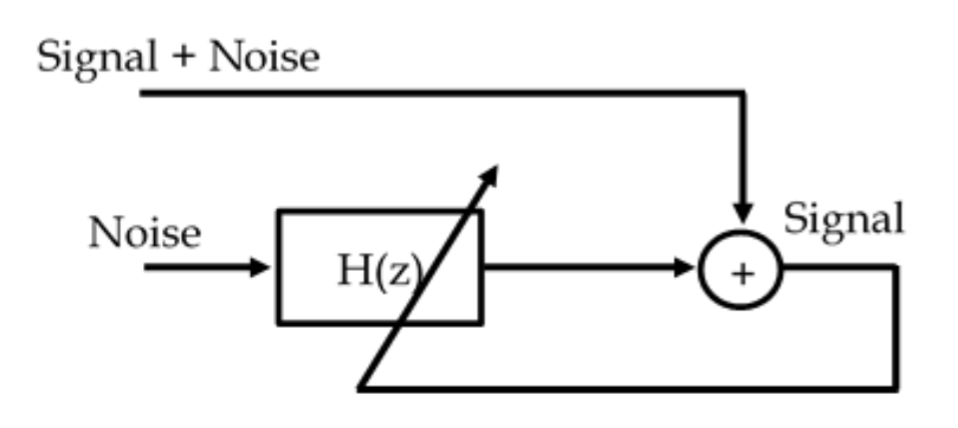
\includegraphics[width=2.5in]{adaptiveFilter}
\caption{Block Diagram for our problem}
\label{modifiedAdaptiveFilter}
\end{figure}
 
 
\begin{figure}
\centering
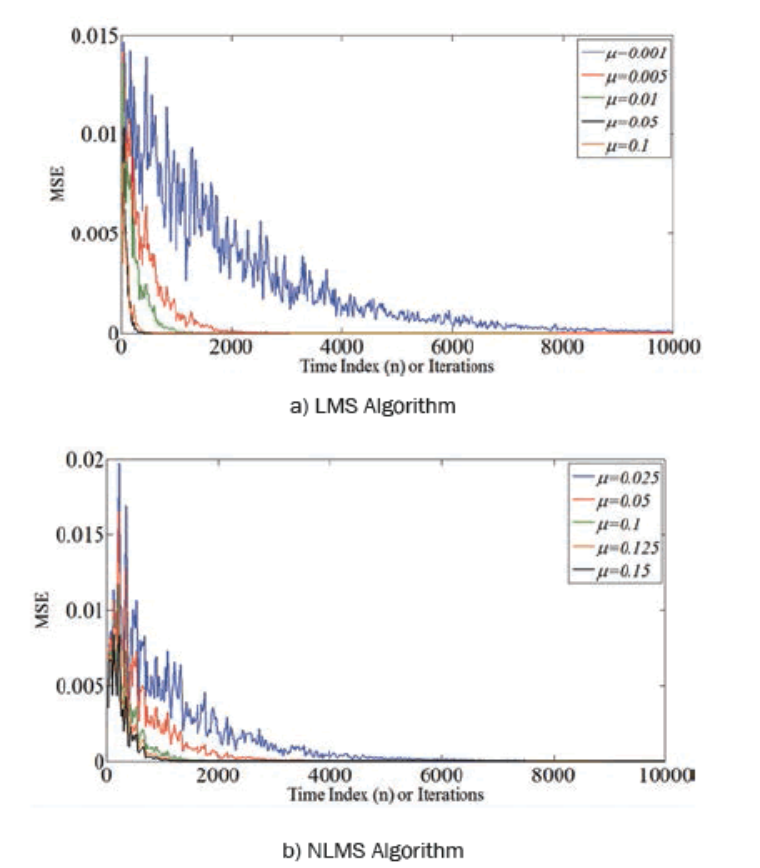
\includegraphics[width=2.5in]{LearningRate}
\caption{Learning Rate for different Step Sizes \cite{SCLIOLEarningRate}}
\label{LearningRatevsStepSize}
\end{figure}
 
 Thus filter's learning rate is thus directly controlled with the step size, this can be seen in the figure \ref{LearningRatevsStepSize}. \cite{SCLIOLEarningRate} As we can see in the figure, as the step size increases, the learning time reduces but the final cost at which the system stops is a little higher than that for the optimal step size. Using a very small step size will reach the point of least cost but it will take a very long time to reach that optimal least cost. Thus using a values in between will reach a cost that is sufficient at well as a shorter delay. This relation between the step size and the learning time can be given by the formula 
 
 $$ \tau = 1 / 4 \times mu \times \lambda_{n} $$
 where $n = 1,2,3,4,5......L$ and $L$ is the order of the filter here.  So choosing the best step size is important.
 
\subsection{Filter Order}
The filter order or the number of taps depend completely on the system under observation. Based on the number of taps or the filter order the step size can be varied to obtain a good learning curve to suit our requirements perfectly. The higher the filter order we will over fit the training data set and it will be disastrous when we try to predict on a completely different testing dataset. The lesser filter order will under fit the data and will also lead to a lot of errors. So the only way to choose the best filter order is with the cross validating across the Training, Validation and Testing Datasets.


\section{Proposed Method}

In our case we are going to slightly modify the signals in the block diagram so that we can understand our problem in case. The modified block diagram can be seen in fig \ref{modifiedAdaptiveFilter}

 As seen from the figure, the signal with the noise(which is the primary in our case) is given as the desired output to the adder while the only noise signal(which is the reference in our case) is given as the input to the adaptive filter.  So this adaptive filter optimizes its parameters to add the speech signal components to the reference to get the primary signal which is the speech with the noise. So the optimized parameters give us the speech components of the signal and hence the error that comes up in the last iteration should be completely free of noise. 

Also for cross validation we have to separate the data into Training Data , Validation Data and Testing Data. The ratio for training validation and testing chosen is 5:1:4 respectively. 

\begin{enumerate}
\item First we run the NLMS algorithm for the training set to learn the weights and then run the same with the validation sets to get the best hyper parameters. Now with the best hyper parameters we run in the testing data set to obtain the voice signal. We can go ahead the test the hyper parameters on the entire data set to obtain the full and complete voice signal.

\item Selecting the step size : In our case the input signal is a realtime online signal and hence calculating the theoretical step size($mu$) is not possible. One way to estimate the theoretical step size would be to wait and collect a huge number of samlpes (ie., 100 samples) and use it to calculate the Eigen spread and estimate the step size. The other way would be to use an educated guess to estimate the step size by letting the algorithm run for a few different step size and filter order combination and choose the combination with which we obtain the least Mean Squared Error, which here is also referred to as the Cost. Once we find the combination which gives us the least cost, we use it to do the other calculations.


\item Selecting the filter order : As explained in the previous subsection, in our case, we let the system run for a couple of different filter order and step size settings and choose the one that gives the least mean squared error.

\end{enumerate}
 
\section{Observations}

For Obesrvation Step 1 the various step sizes used for setup are $[0.01:0.01:0.5]$, the various filter orders used in this setup are $[2,8,10,20,25,30,32,36,38,40,44,46,48,50,55,60,65]$.  For Observation Step 2 the various step sizes used for setup are $[0.01:0.01:0.3]$, the various filter orders used in this setup are $[10,20,50]$. First, we train the system and then validate the system to obtain the best hyper parameters. 

\subsection{Observation Set 1}

\begin{enumerate} 


\begin{figure*}
\centering
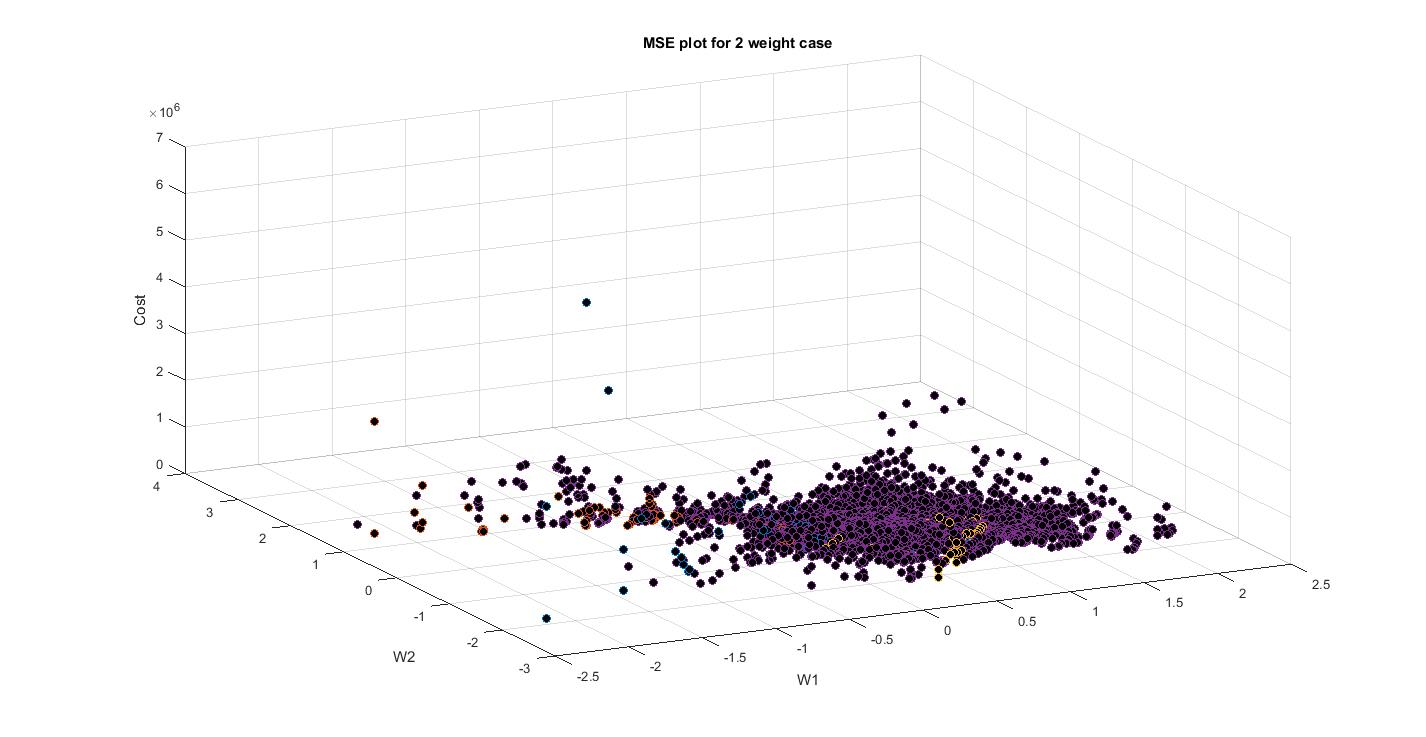
\includegraphics[scale=0.40]{MSEPlotFor2WeightCase_View1.jpg}
%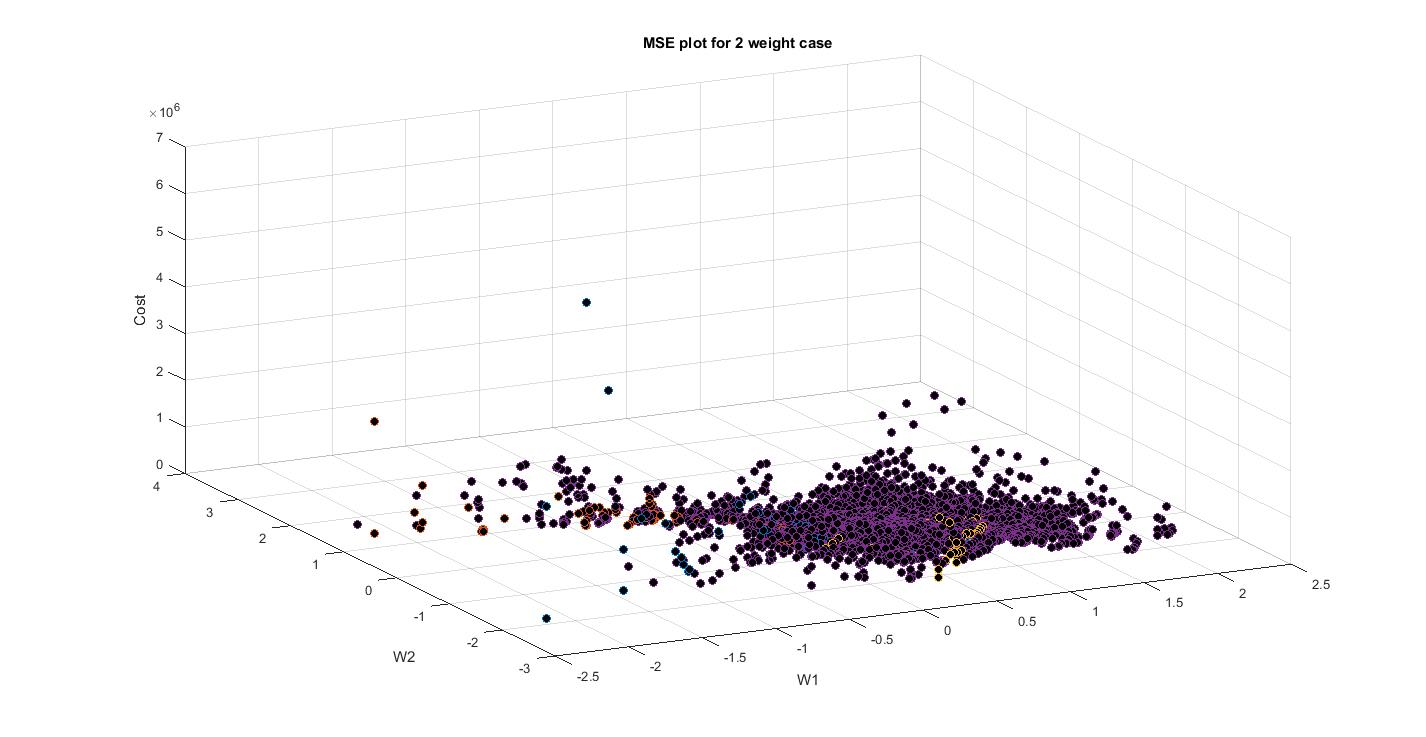
\includegraphics{MSEPlotFor2WeightCase_View1.jpg}
\caption{MSE plot for 2 Weight Case View 1}
\label{MSE2wt_v1}
\end{figure*}

\begin{figure*}
\centering
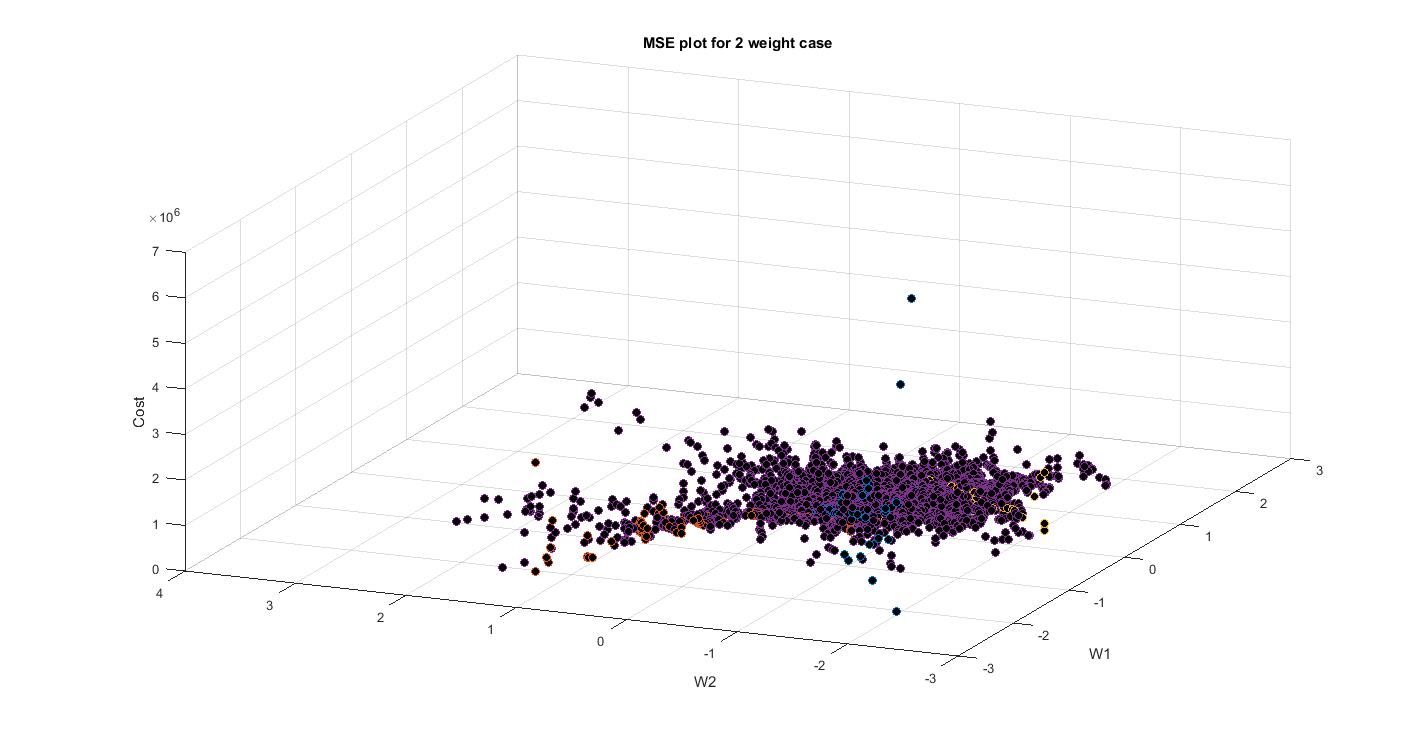
\includegraphics[scale=0.40]{MSEPlotFor2WeightCase_View2.jpg}
\caption{MSE plot for 2 Weight Case View 2}
\label{MSE2wt_v2}
\end{figure*}






\item Two weight case : In this case we specify the filter order as 2. We choose the step size as 0.1 and calculate MSE for the different weights.  To plot the MSE vs W1 vs W2 plot. We first run the NLMS algorithm with the above mentioned hyper parameters and then get the different W1 and W2s. Now we check the limit of the the weights. and then discretize the range so that it becomes computationally do-able and then calculate the cost train for the different weights. This gives us a cost train for the different weight starting point. Thus plotting a line plot for each of the cost train we find that the system runs in a way to reduce the cost and chooses a weight train that reduces the cost. This explains the adaptive nature of the filter.  The figures \ref{MSE2wt_v2} \&\ref{MSE2wt_v1} are the 2 different views of the plots. The 2 views are provided for better understanding of the plot surface. \\

From the figures \ref{MSE2wt_v1} \& \ref{MSE2wt_v2} we can see that , even when we start at different points in the weight surface we tend to converge at the cluster (where we have a lot of points). Also this would look like a concave surface if the points were replaced by a plane. With the concave facing upwards. The cluster is also referred to as the local minimum or global minimum in this case. That is the point where we obtain the least cost.  We can also understand that the weights converge at the local minimum. This has been plotted for 30000 iterations so it also shows that it needs around 30000 iterations for attaining the local minimum. But in the case of higher order which will be explained in the further sections we can see that we will attain the local minimum at around 50 iterations itself. This is the MSE surface for the 2 weight case for our problem. 

The figure \ref{WvsIterations} gives us the different values of W1 and W2 over iterations. \\

\begin{figure*}
\centering
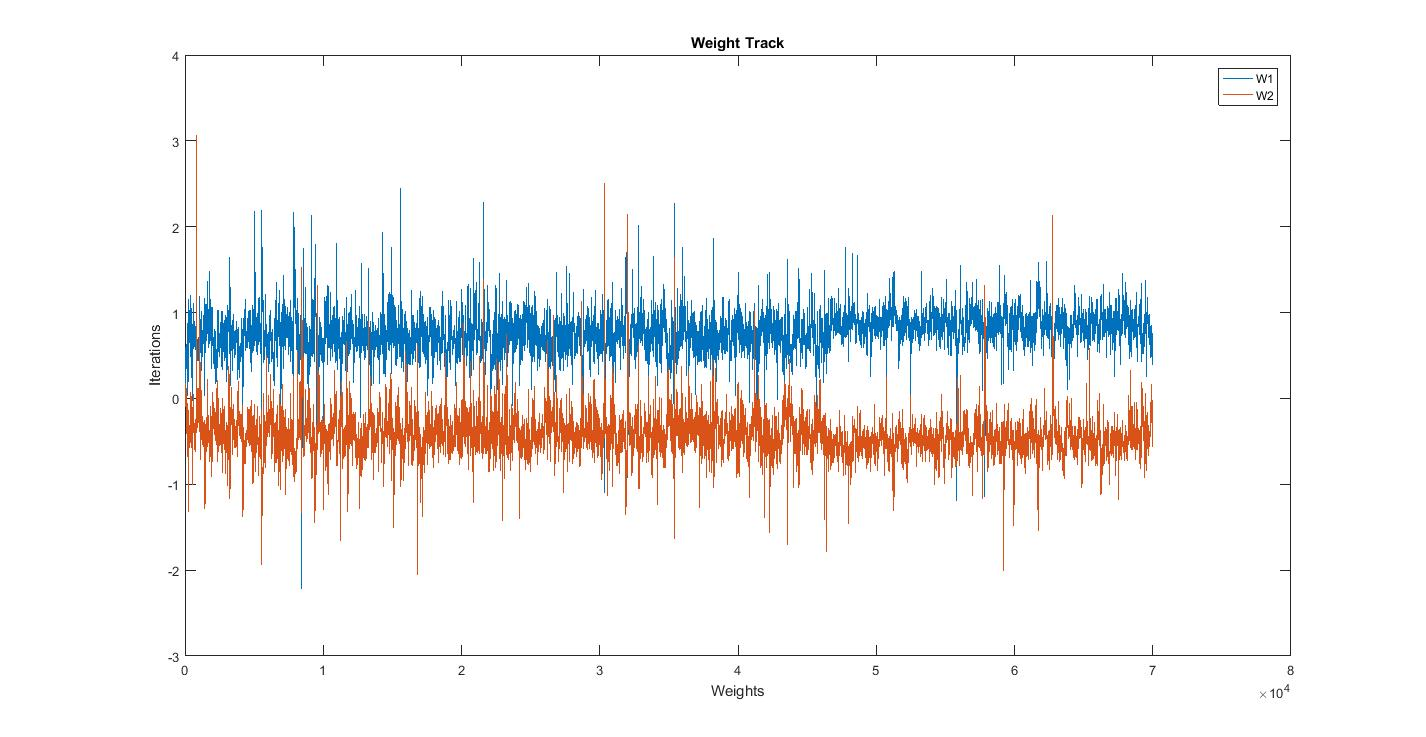
\includegraphics[scale=0.40]{WeightTrackFor2WeightCase.jpg}
\caption{WeightTracks Over Iterations}
\label{WvsIterations}
\end{figure*}

\item The learning curve for different step size $mu$ has been plot and is available in the figure \ref{LearningCurve_1}. This figure \ref{LearningCurve_1} is a zoom into the learning curve to actually see where we obtain the first convergence . From the learning curve we can observe the following 
\begin{enumerate}

\item For higher step size $mu=0.27$ the learning curve converges in less than 5 iterations but for lower step sizes of $mu=0.20$ \& $mu=-0.02$ the filter converges at around 15 and 50+ iterations respectively. This confirms our proof that learning rate is quicker at higher step sizes and slower at lower step sizes. 

\item Their oscillations around the mean point can be seen in the next set of figure \ref{LearningCurve_pt02}, \ref{LearningCurve_pt20} \& \ref{LearningCurve_pt28}. Also we can clearly see that for higher step size the curve converges sooner. \\

\end{enumerate} 
\begin{figure*}
\centering
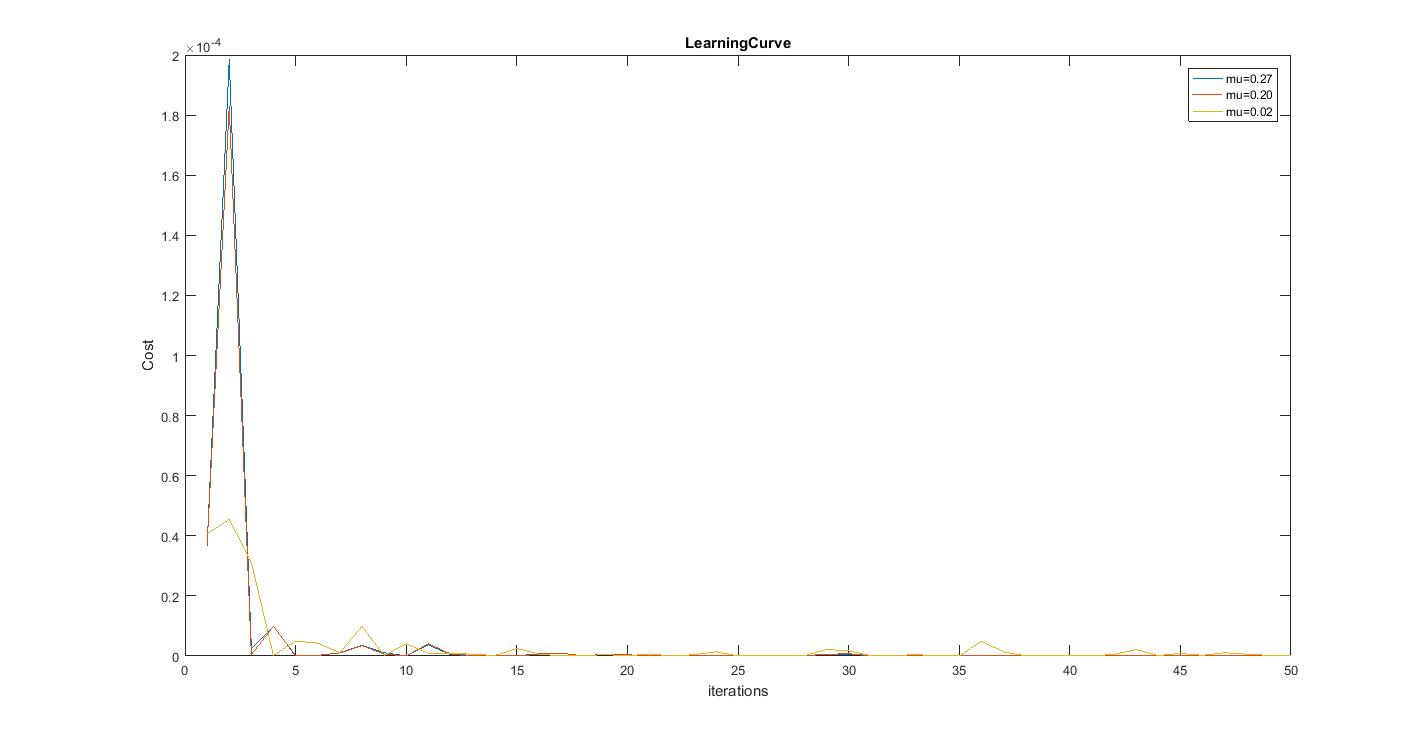
\includegraphics[scale=0.40]{LearningCurvetraining.jpg}
\caption{Learning Curve zoomed in for 50 iterations}
\label{LearningCurve_1}
\end{figure*}


\begin{figure*}
\centering
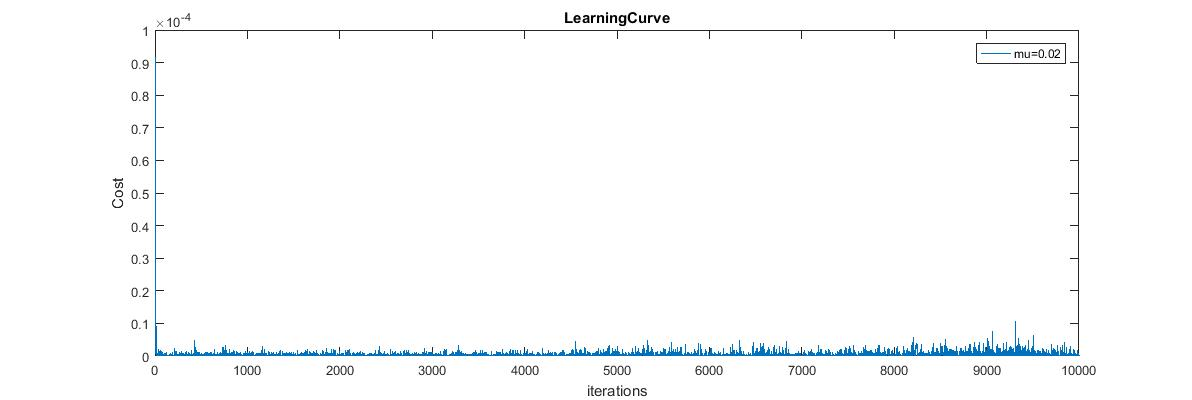
\includegraphics[scale=0.40]{LearningCurve_mupt02.jpg}
\caption{LearningCurve for mu = 0.02}
\label{LearningCurve_pt02}
\end{figure*}

\begin{figure*}
\centering
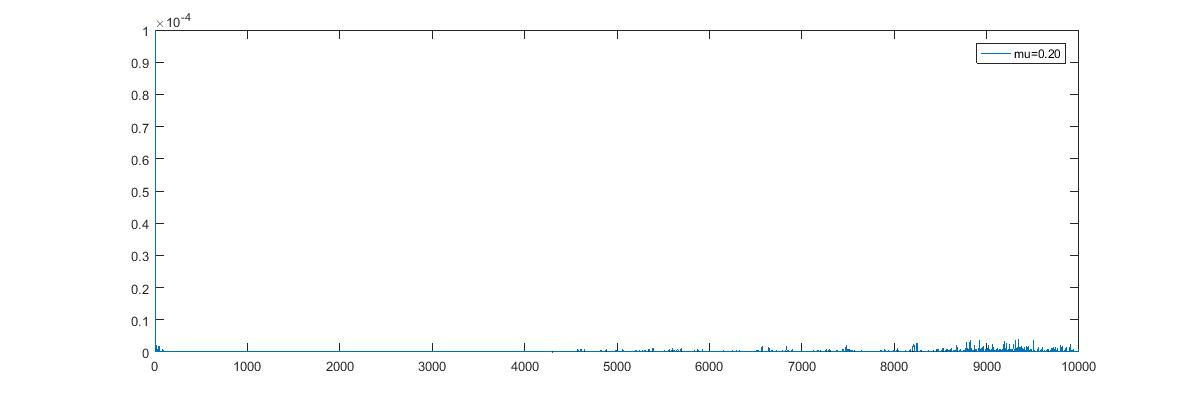
\includegraphics[scale=0.40]{LearningCurve_mupt20.jpg}
\caption{LearningCurvefor mu = 0.20}
\label{LearningCurve_pt20}
\end{figure*}

\begin{figure*}
\centering
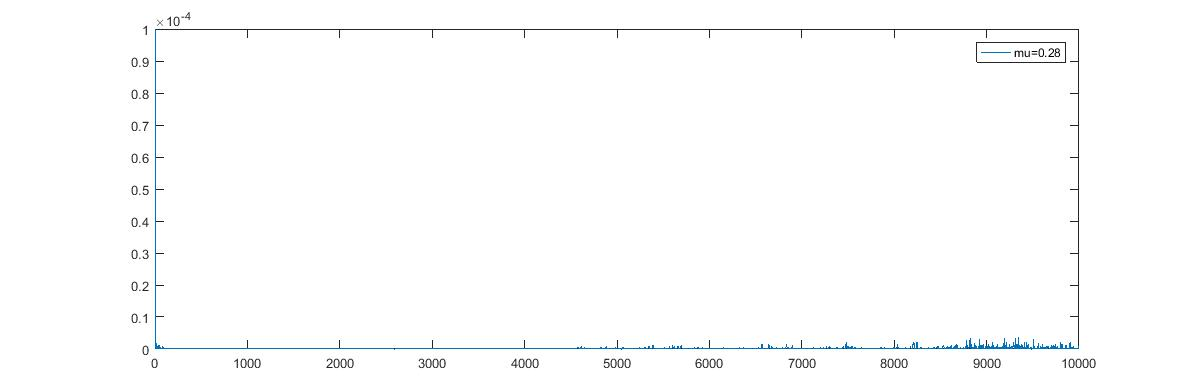
\includegraphics[scale=0.40]{LearningCurve_mupt28.jpg}
\caption{LearningCurve for mu = 0.28}
\label{LearningCurve_pt28}
\end{figure*}

\item We calculate the ERLE(Echo Return Loss Enhancement) improvement to measure the quality of the voice signal we obtain for the given input and the desired output for different hyper parameters and plot the ERLE vs step size and filter order. This plot is available in figure \ref{ERLE Plot}. This figure also shows us that the hyper parameters chosen for the system can also be chosen from this plot. The point of highest dB coincides with point of minimum error of the MSE plot which is available in the figure \ref{MSE Plot}. We get the best performance with filter order 48 and step size 0.25 for our system. We can filter the signal for any local impulse response and remove any jitter or vibrations before calculating the plot.

The ERLE was calculated using the formula 

$$ERLE = 10 log_{10}( Power of Desired Signal /  Power of Noise )$$

The best mean ERLE obtained was 21.9740. The best SNR improvement or  best variance or ERLE obtained was 30.96 . These were also the optimum points of hyper parameters. \\

The voice signal is "I will not condone a course of action that will lead us to war" \\


\begin{figure*}
\centering
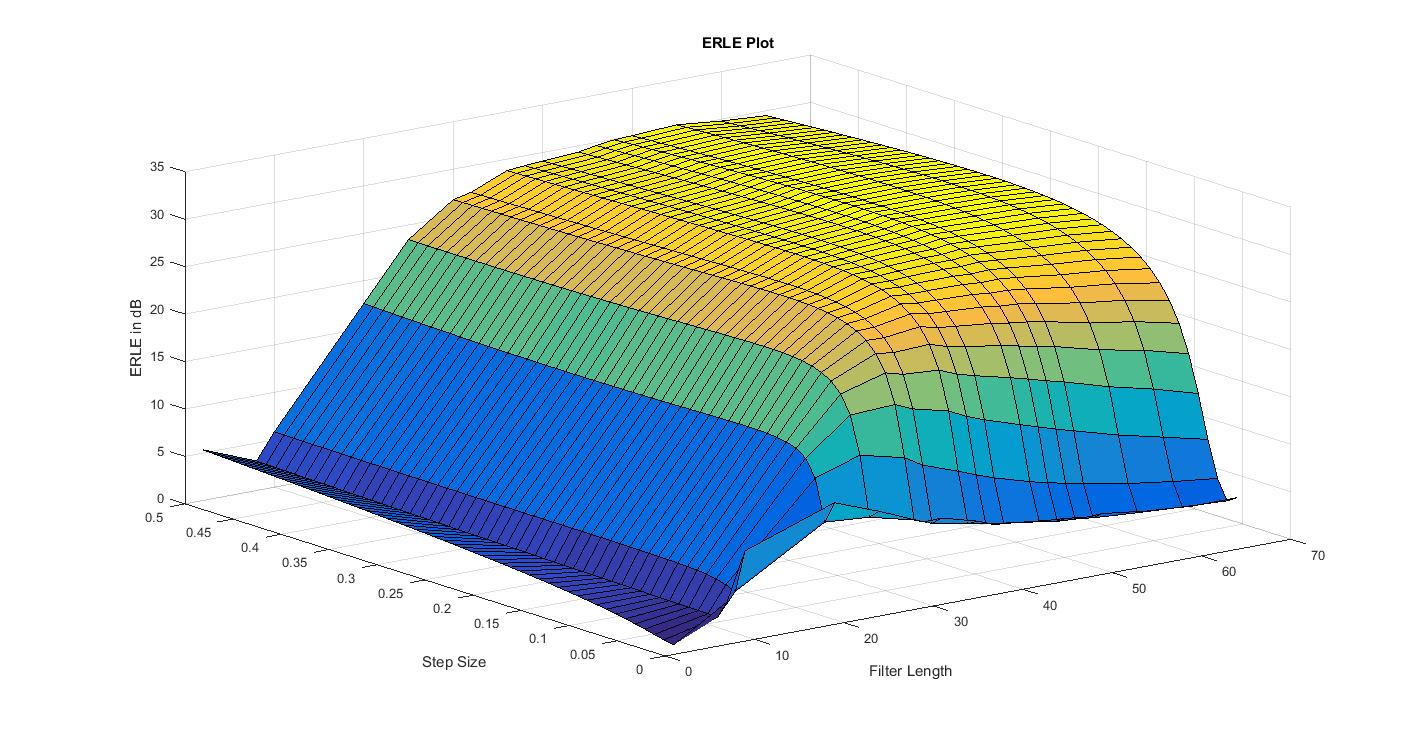
\includegraphics[scale=0.40]{ERLEPlot_training.jpg}
\caption{ERLE vs Hyperparameters}
\label{ERLE Plot}
\end{figure*}


\begin{figure*}
\centering
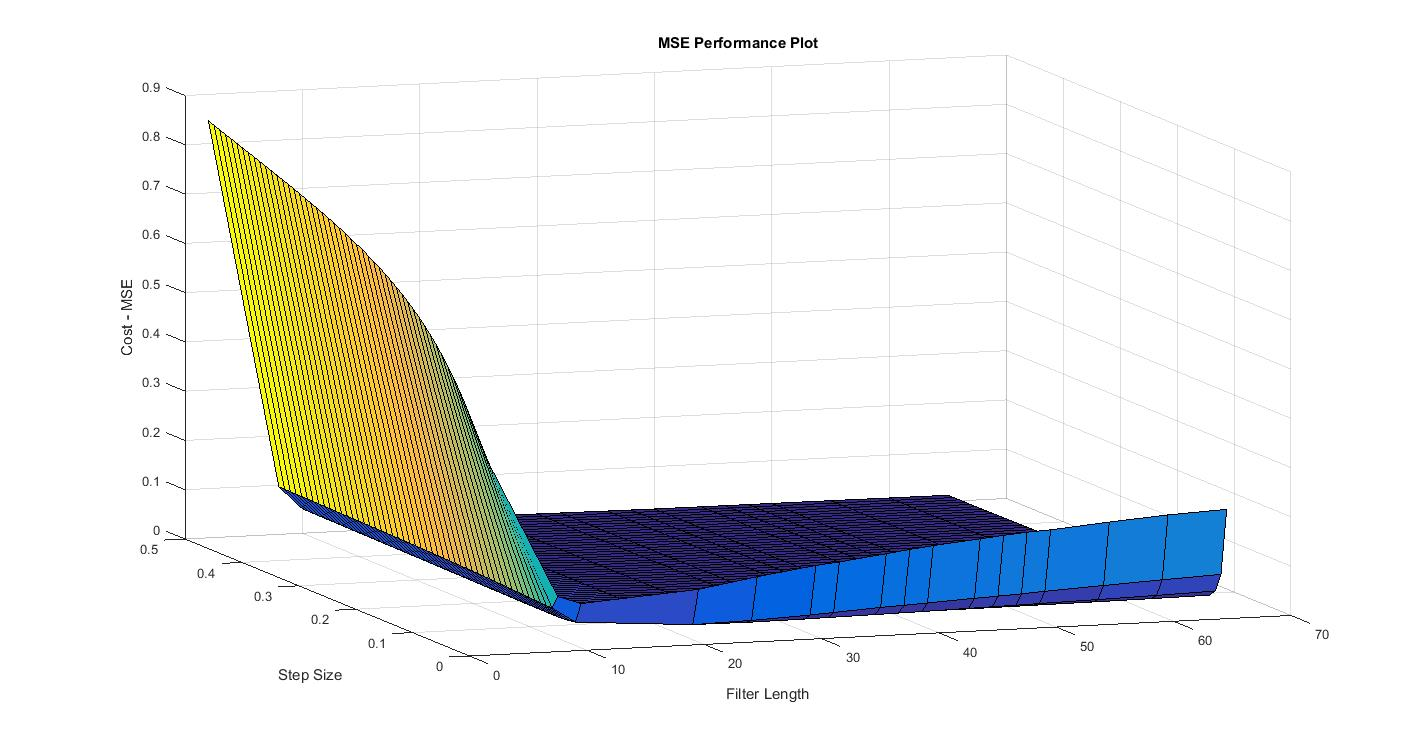
\includegraphics[scale=0.40]{MSEPlot.jpg}
\caption{MSE vs Hyperparameters}
\label{MSE Plot}
\end{figure*}

\end{enumerate}
\subsection{Observation Set 2}

Improving the performance by improving the filter order is accepted but, it may lead to over fitting of the trained data. In real time the data we obtain for training and testing is not going to be similar and may vary and hence if we have over-fitted it, it will cause high error rates, but in our case as the training and testing is of the same signal type obtained from the same source overfitting will not be a problem up-to a level. \\

Yes we can cross validate based on ERLE, this has been explained in the observation 3 in observation set 1. The ERLE plot can be used similar to the MSE performance surface plot but, we will have to choose a point of maximum ERLE change compared to the lowest point in MSE surface plot. The plots are available in figures \ref{MSE Plot} \& \ref{ERLE Plot}.

\begin{enumerate}
\item The plot for the filter orders of 20, 30, and 50 against different step sizes vs MSE is available in figure \ref{ERLE Plot2}. From the plot we can see that as the filter order increases the performance increases(ERLE increases).

\begin{figure*}
\centering
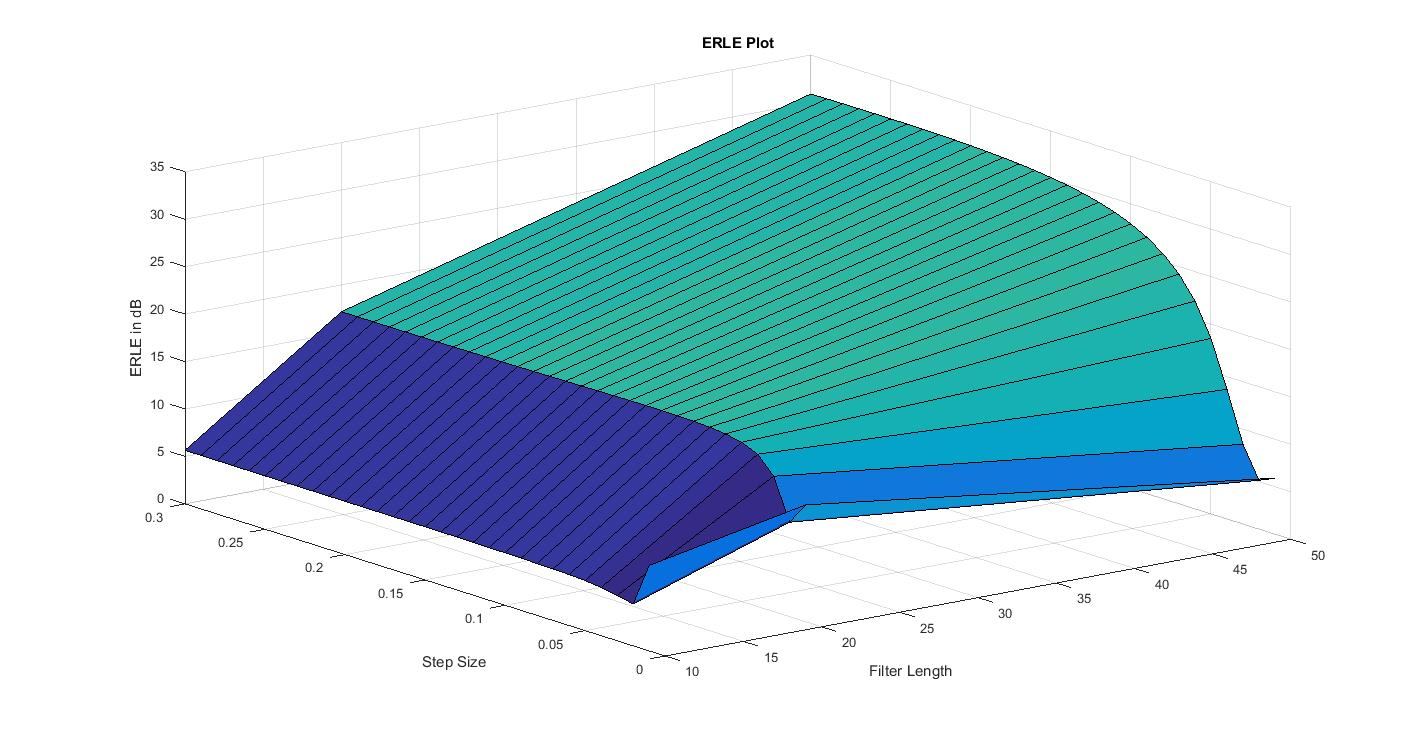
\includegraphics[scale=0.40]{ERLEPlot2-3.jpg}
\caption{ERLE for Filter Order 10 , 20 and 50}
\label{ERLE Plot2}
\end{figure*}
\begin{figure*}
\centering
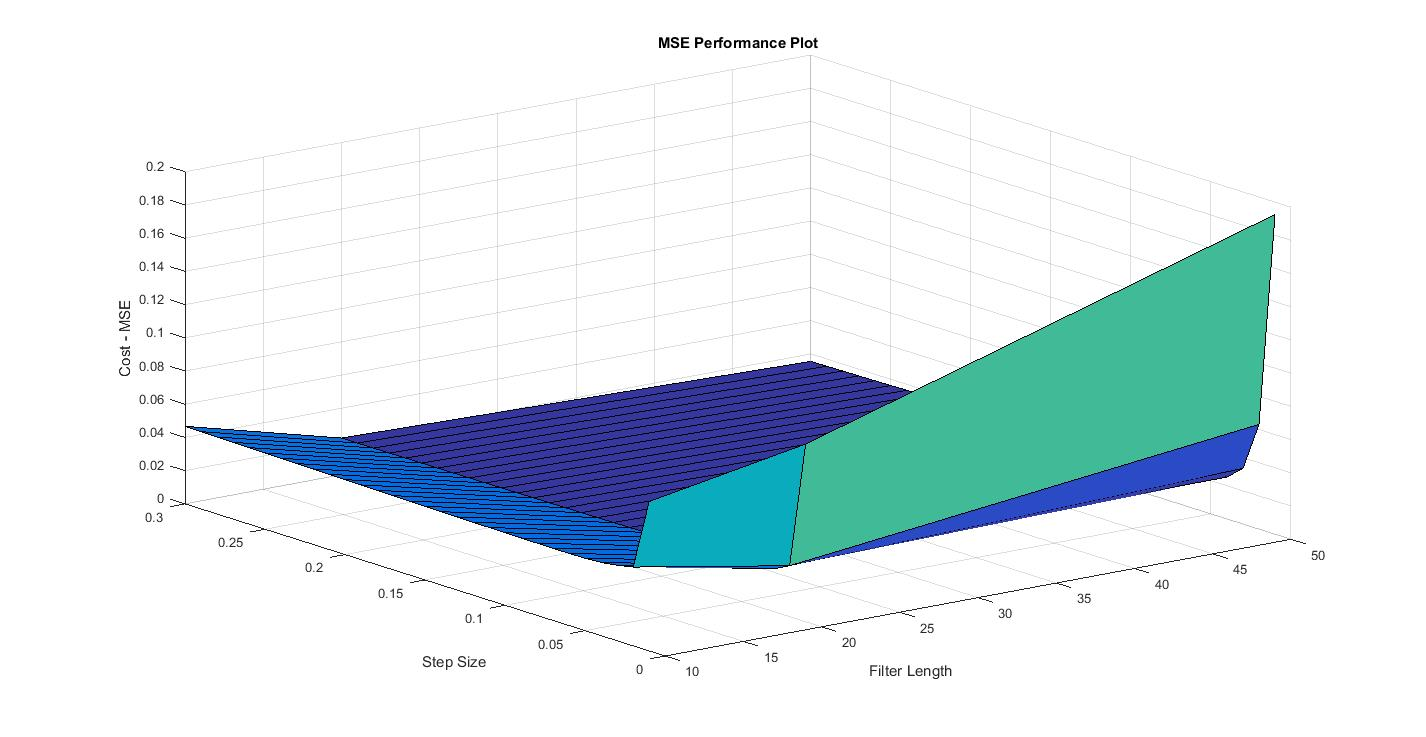
\includegraphics[scale=0.40]{MSEPlot2.jpg}
\caption{ERLE for Filter Order 10 , 20 and 50}
\label{MSE Plot2}
\end{figure*}

Looking at the plot we get maximum change in ERLE of 30.9439 at $step size = 0.26$ and $filter order = 50$ which is similar to the hyper-parameters we obtain in the MSE plot which is available in figure \ref{MSE Plot2}

\item We get the best performance at step size = 0.26 which is little lesser than that for filter order 48 which we had chosen as our optimal parameter. This again proves the point that increasing the filter order we can increase the performance (but might lead to overfitting). The learning curve for the best performance and the 2 other learning curves for comparison are provided in figures \ref{LearningCurve_pt02_order50} \ref{LearningCurve_pt17_order50} \ref{LearningCurve_pt26_order50}. A zoomed version of it is available in \ref{LearningCurve_zoom_order50}, we can see that this is very similar to the one obtained in the observation set 1.

\begin{figure*}
\centering
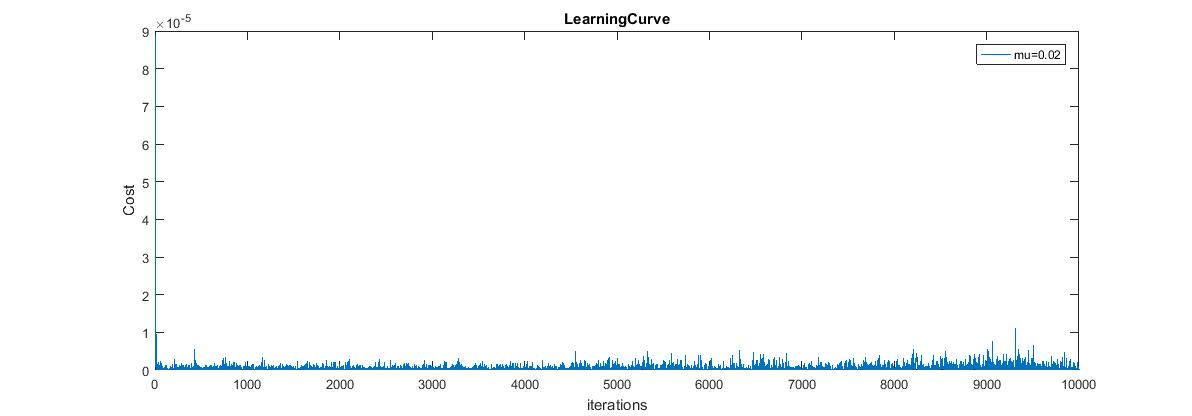
\includegraphics[scale=0.40]{LearningCurve_mupt02_order50.jpg}
\caption{ Learning Curve Filter order 50 mu 0.02}
\label{LearningCurve_pt02_order50}
\end{figure*}
\begin{figure*}
\centering
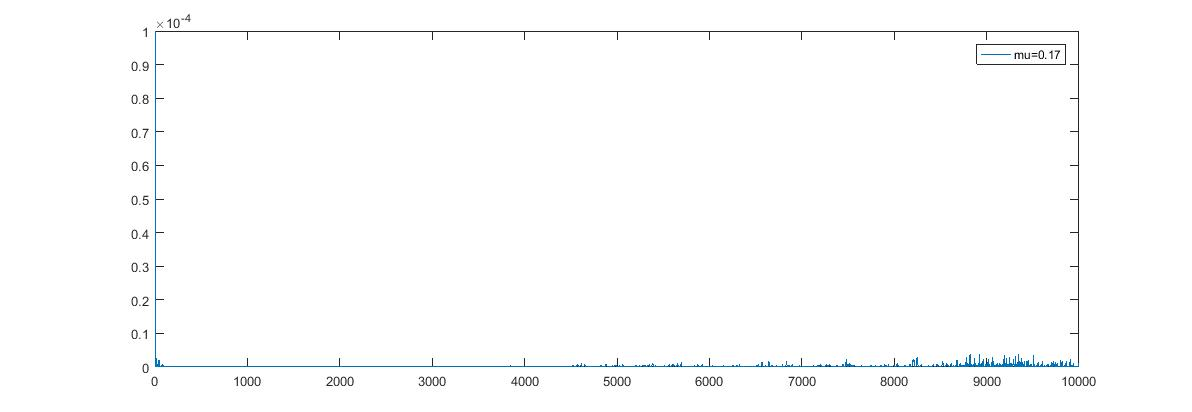
\includegraphics[scale=0.40]{LearningCurve_mupt17_order50.jpg}
\caption{ Learning Curve Filter order 50 mu 0.17}
\label{LearningCurve_pt17_order50}
\end{figure*}
\begin{figure*}
\centering
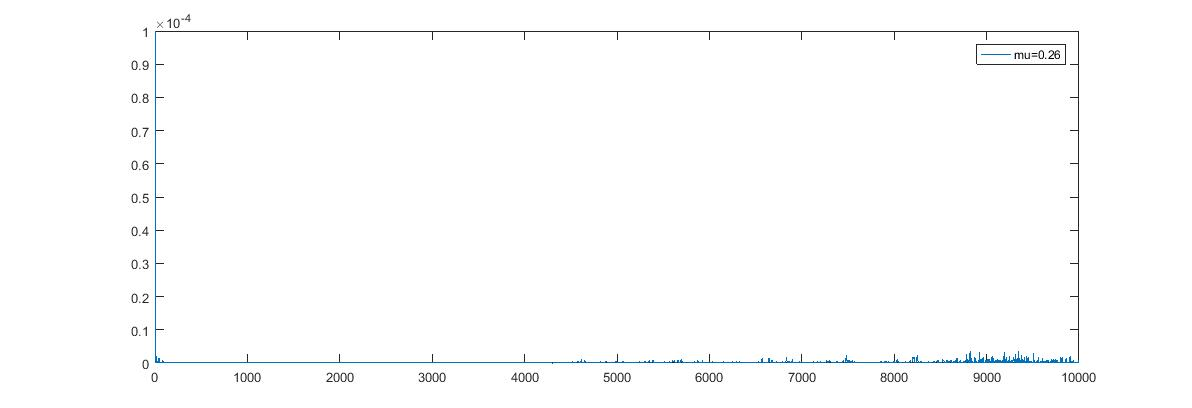
\includegraphics[scale=0.40]{LearningCurve_mupt26_order50.jpg}
\caption{ Learning Curve Filter order 50 mu 0.26}
\label{LearningCurve_pt26_order50}
\end{figure*}


\begin{figure*}
\centering
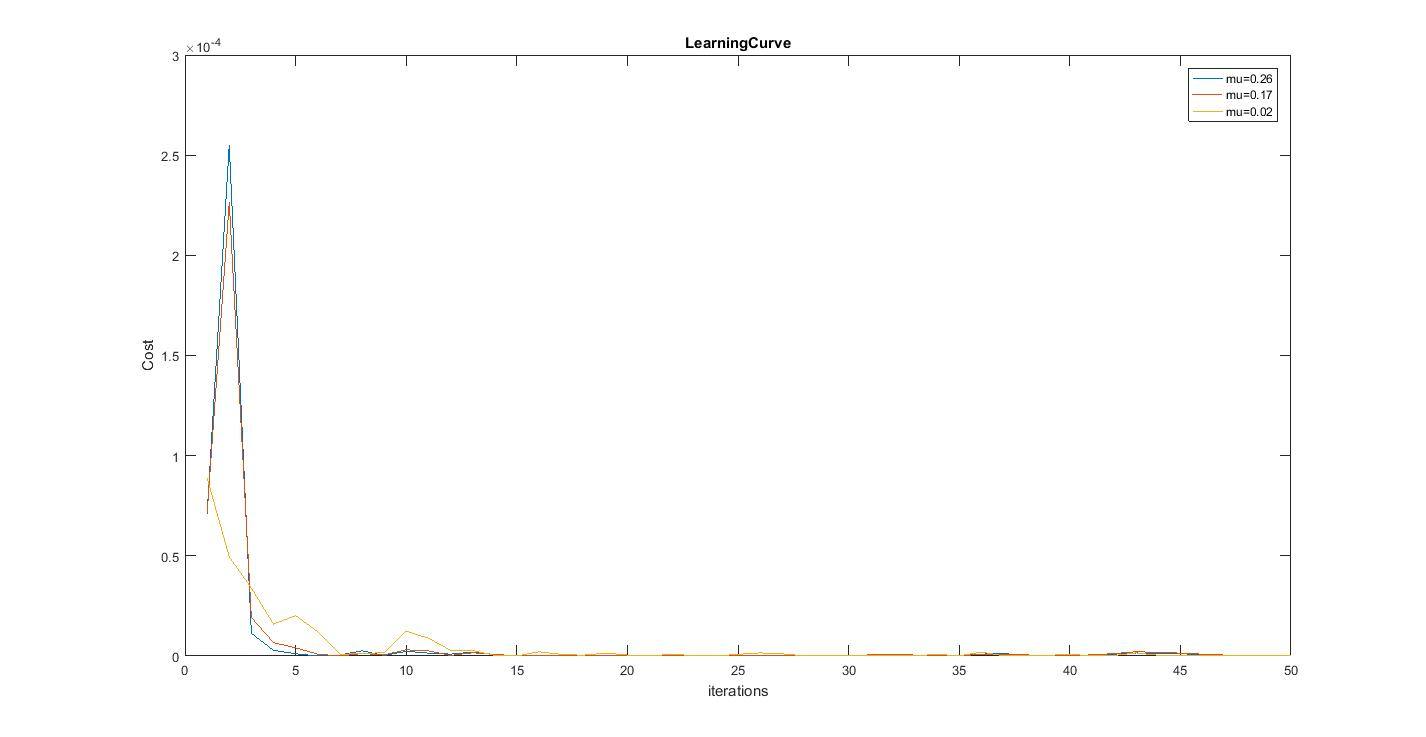
\includegraphics[scale=0.40]{LearningCurve_order50.jpg}
\caption{ Learning Curve zoomed in for Order 50}
\label{LearningCurve_zoom_order50}
\end{figure*}


\item The best filter does give the best speech intelligibility. The speech signal is obtained at the very least order itself but it still has a component of noise in it. As we increase the filter order the speech intelligibility increases and the vacuum cleaner noise reduces( it is as though the noise moves further away from the voice signal). Thus best voice signal is obtained in the filter order 50 in our second observation. 

\end{enumerate}


% An example of a floating figure using the graphicx package.
% Note that \label must occur AFTER (or within) \caption.
% For figures, \caption should occur after the \graphics.
% Note that IEEEtran v1.7 and later has special internal code that
% is designed to preserve the operation of \label within \caption
% even when the captionsoff option is in effect. However, because
% of issues like this, it may be the safest practice to put all your
% \label just after \caption rather than within \caption{}.
%
% Reminder: the "draftcls" or "draftclsnofoot", not "draft", class
% option should be used if it is desired that the figures are to be
% displayed while in draft mode.
%
%\begin{figure}[!t]
%\centering
%\includegraphics[width=2.5in]{myfigure}
% where an .eps filename suffix will be assumed under latex, 
% and a .pdf suffix will be assumed for pdflatex; or what has been declared
% via \DeclareGraphicsExtensions.
%\caption{Simulation results for the network.}
%\label{fig_sim}
%\end{figure}

% Note that the IEEE typically puts floats only at the top, even when this
% results in a large percentage of a column being occupied by floats.


% An example of a double column floating figure using two subfigures.
% (The subfig.sty package must be loaded for this to work.)
% The subfigure \label commands are set within each subfloat command,
% and the \label for the overall figure must come after \caption.
% \hfil is used as a separator to get equal spacing.
% Watch out that the combined width of all the subfigures on a 
% line do not exceed the text width or a line break will occur.
%
%\begin{figure*}[!t]
%\centering
%\subfloat[Case I]{\includegraphics[width=2.5in]{box}%
%\label{fig_first_case}}
%\hfil
%\subfloat[Case II]{\includegraphics[width=2.5in]{box}%
%\label{fig_second_case}}
%\caption{Simulation results for the network.}
%\label{fig_sim}
%\end{figure*}
%
% Note that often IEEE papers with subfigures do not employ subfigure
% captions (using the optional argument to \subfloat[]), but instead will
% reference/describe all of them (a), (b), etc., within the main caption.
% Be aware that for subfig.sty to generate the (a), (b), etc., subfigure
% labels, the optional argument to \subfloat must be present. If a
% subcaption is not desired, just leave its contents blank,
% e.g., \subfloat[].


% An example of a floating table. Note that, for IEEE style tables, the
% \caption command should come BEFORE the table and, given that table
% captions serve much like titles, are usually capitalized except for words
% such as a, an, and, as, at, but, by, for, in, nor, of, on, or, the, to
% and up, which are usually not capitalized unless they are the first or
% last word of the caption. Table text will default to \footnotesize as
% the IEEE normally uses this smaller font for tables.
% The \label must come after \caption as always.
%
%\begin{table}[!t]
%% increase table row spacing, adjust to taste
%\renewcommand{\arraystretch}{1.3}
% if using array.sty, it might be a good idea to tweak the value of
% \extrarowheight as needed to properly center the text within the cells
%\caption{An Example of a Table}
%\label{table_example}
%\centering
%% Some packages, such as MDW tools, offer better commands for making tables
%% than the plain LaTeX2e tabular which is used here.
%\begin{tabular}{|c||c|}
%\hline
%One & Two\\
%\hline
%Three & Four\\
%\hline
%\end{tabular}
%\end{table}


% Note that the IEEE does not put floats in the very first column
% - or typically anywhere on the first page for that matter. Also,
% in-text middle ("here") positioning is typically not used, but it
% is allowed and encouraged for Computer Society conferences (but
% not Computer Society journals). Most IEEE journals/conferences use
% top floats exclusively. 
% Note that, LaTeX2e, unlike IEEE journals/conferences, places
% footnotes above bottom floats. This can be corrected via the
% \fnbelowfloat command of the stfloats package.




\section{Conclusion}
\begin{enumerate}
\item The Normalized LMS converges much faster than the LMS algorithm
\item The voice signal is separated and it is from the famous movie Star Wars Episode 1- Phantom Menace "I will not condone a course of action that will lead us to war". 
\item ERLE ; Filter order 10 step size 0.26 = 5.6255 
\item ERLE ; Filter order 20 step size 0.26 = 17.1791 
\item ERLE ;  Filter order 50 step size 0.26 = 30.9439 
\item ERLE ;  Filter order 48 step size 0.25 = 30.9686 , This is also the optimal point for our hyper parameters.


\end{enumerate}




% conference papers do not normally have an appendix


% use section* for acknowledgment






% trigger a \newpage just before the given reference
% number - used to balance the columns on the last page
% adjust value as needed - may need to be readjusted if
% the document is modified later
%\IEEEtriggeratref{8}
% The "triggered" command can be changed if desired:
%\IEEEtriggercmd{\enlargethispage{-5in}}

% references section

% can use a bibliography generated by BibTeX as a .bbl file
% BibTeX documentation can be easily obtained at:
% http://mirror.ctan.org/biblio/bibtex/contrib/doc/
% The IEEEtran BibTeX style support page is at:
% http://www.michaelshell.org/tex/ieeetran/bibtex/
%\bibliographystyle{IEEEtran}
% argument is your BibTeX string definitions and bibliography database(s)
%\bibliography{IEEEabrv,../bib/paper}
%
% <OR> manually copy in the resultant .bbl file
% set second argument of \begin to the number of references
% (used to reserve space for the reference number labels box)
\begin{thebibliography}{1}

\bibitem{AdaptiveNoiseCancelling1975}
B. Widrow et al., "Adaptive noise cancelling: Principles and applications," in Proceedings of the IEEE, vol. 63, no. 12, pp. 1692-1716, Dec. 1975.
doi: 10.1109/PROC.1975.10036

\bibitem{Howells_SideLobeCanceller}
P. Howells, ?Intermediatefrequency side-lobe canceller,? U S .
Patent 3 202 990, Aug. 24,1965

\bibitem{WidrowHoffdaptiveSwitching}
B. Widrow and M. Hoff, Jr., ?Adaptive switching circuits,? in
IRE WESCON Conv. Rec., pt. 4, pp. 96-104,1960.

\bibitem{McgrawhillNilssonLearningMachines}
N.Nilsson ,LearningMachines. New York: McGraw-Hill,1965

\bibitem{GloverAdaptiveNoiseCancelling}
J. Glover, "Adaptive noise canceling applied to sinusoidal interferences," in IEEE Transactions on Acoustics, Speech, and Signal Processing, vol. 25, no. 6, pp. 484-491, Dec 1977

\bibitem{SCLIOLEarningRate}
JIMENEZ-LOPEZ, Fabi�n Rolando; PARDO-BEAINY, Camilo Ernesto  and  GUTIERREZ-CACERES, Edgar Andr�s. Adaptive filtering implemented over TMS320c6713 DSP platform for system identification. Iteckne [online]. 2014, vol.11, n.2 [cited  2016-10-14], pp.157-171

\end{thebibliography}




% that's all folks
\end{document}


